\documentclass[aspectratio=169,11pt]{beamer}\usetheme{default}\usecolortheme{seahorse}\setbeamertemplate{navigation symbols}{}\setbeamertemplate{footline}[frame number]
\usepackage[T1]{fontenc}\usepackage[utf8]{inputenc}\usepackage{helvet}\usepackage{booktabs}
\title{How wide is rue de Terrebonne?}\subtitle{The roadway along the lane, measured on the City\textquoteright{}s 2015 LiDAR}\author{Terrebonne-open-sources (a resident of Côte-des-Neiges--Notre-Dame-de-Grâce)}\date{2026-11-04}
\begin{document}
\begin{frame}\titlepage\end{frame}
\begin{frame}{The question}\begin{itemize}
\item The winter layout adopted on November 2, 2026 (file 1266880005) turns the lane running with traffic into parking and has cyclists share the traffic lane.
\item The borough\textquoteright{}s 2023 study drew that type of section (EXP, Fig.~6-6): parking 2.4 + shared lane 3.5 + parking 2.4 + buffer 0.5 + contraflow lane 2.0 = \textbf{10.8 m} curb to curb.
\item Is the street 10.8 m wide, everywhere along its 2.4 km? That decides how much room any winter layout has.
\end{itemize}\vfill\scriptsize Source: EXP 2023, p.~72; borough file 1266880005, pp.~207--212 of the Nov.~2 bundle.\end{frame}
\begin{frame}{Data and method}\begin{itemize}
\item Ville de Montréal, LiDAR aérien 2015 (open data, CC-BY 4.0): ground returns averaged on a 0.25 m grid along the corridor.
\item A cross-section every 2 m along the lane\textquoteright{}s axis (1207 stations), 16 m each side, every 0.1 m.
\item Curb = the first rise of 7 cm over 0.5 m outward from the axis, 3--8 m out (a curb face is 10--15 cm; a 1:12 driveway ramp rises 4 cm and does not pass).
\item Night flight, cars at the curbs: no ground under a car. Stations with both curbs found and a width of 9--13 m are kept: 759.
\item Right-of-way: parcel line to parcel line on the same section (City assessment units).
\end{itemize}\end{frame}
\begin{frame}{The roadway is 11.0 m wide, along the whole street}\centering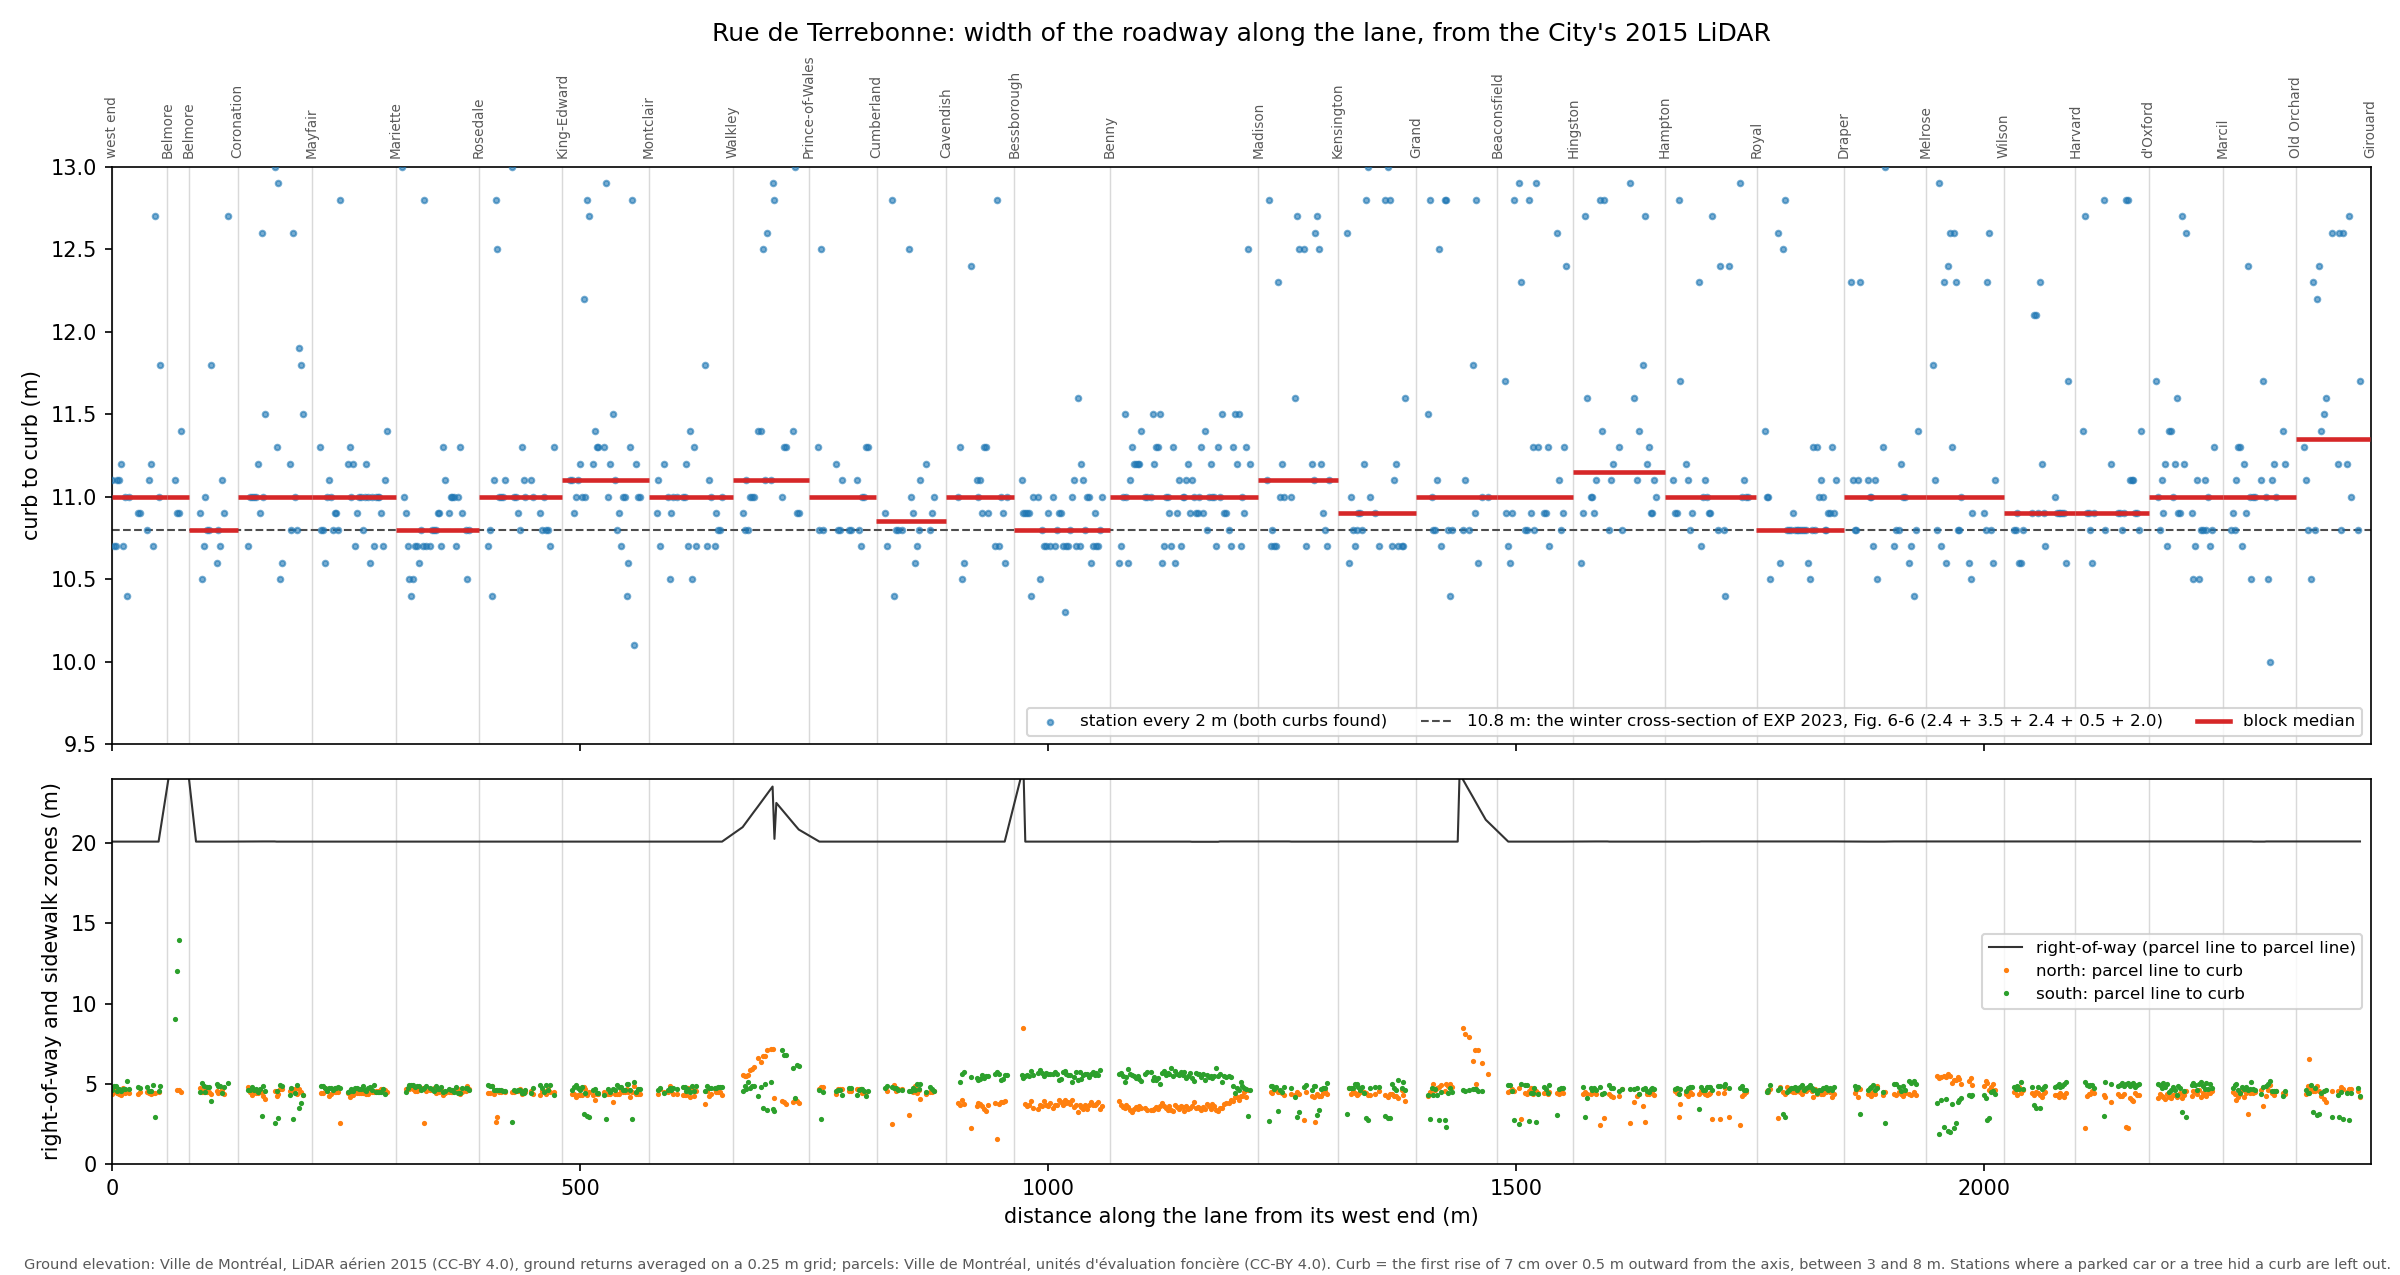
\includegraphics[width=\textwidth]{figures/street_width_profile_en.png}\end{frame}
\begin{frame}{What a cross-section looks like}\centering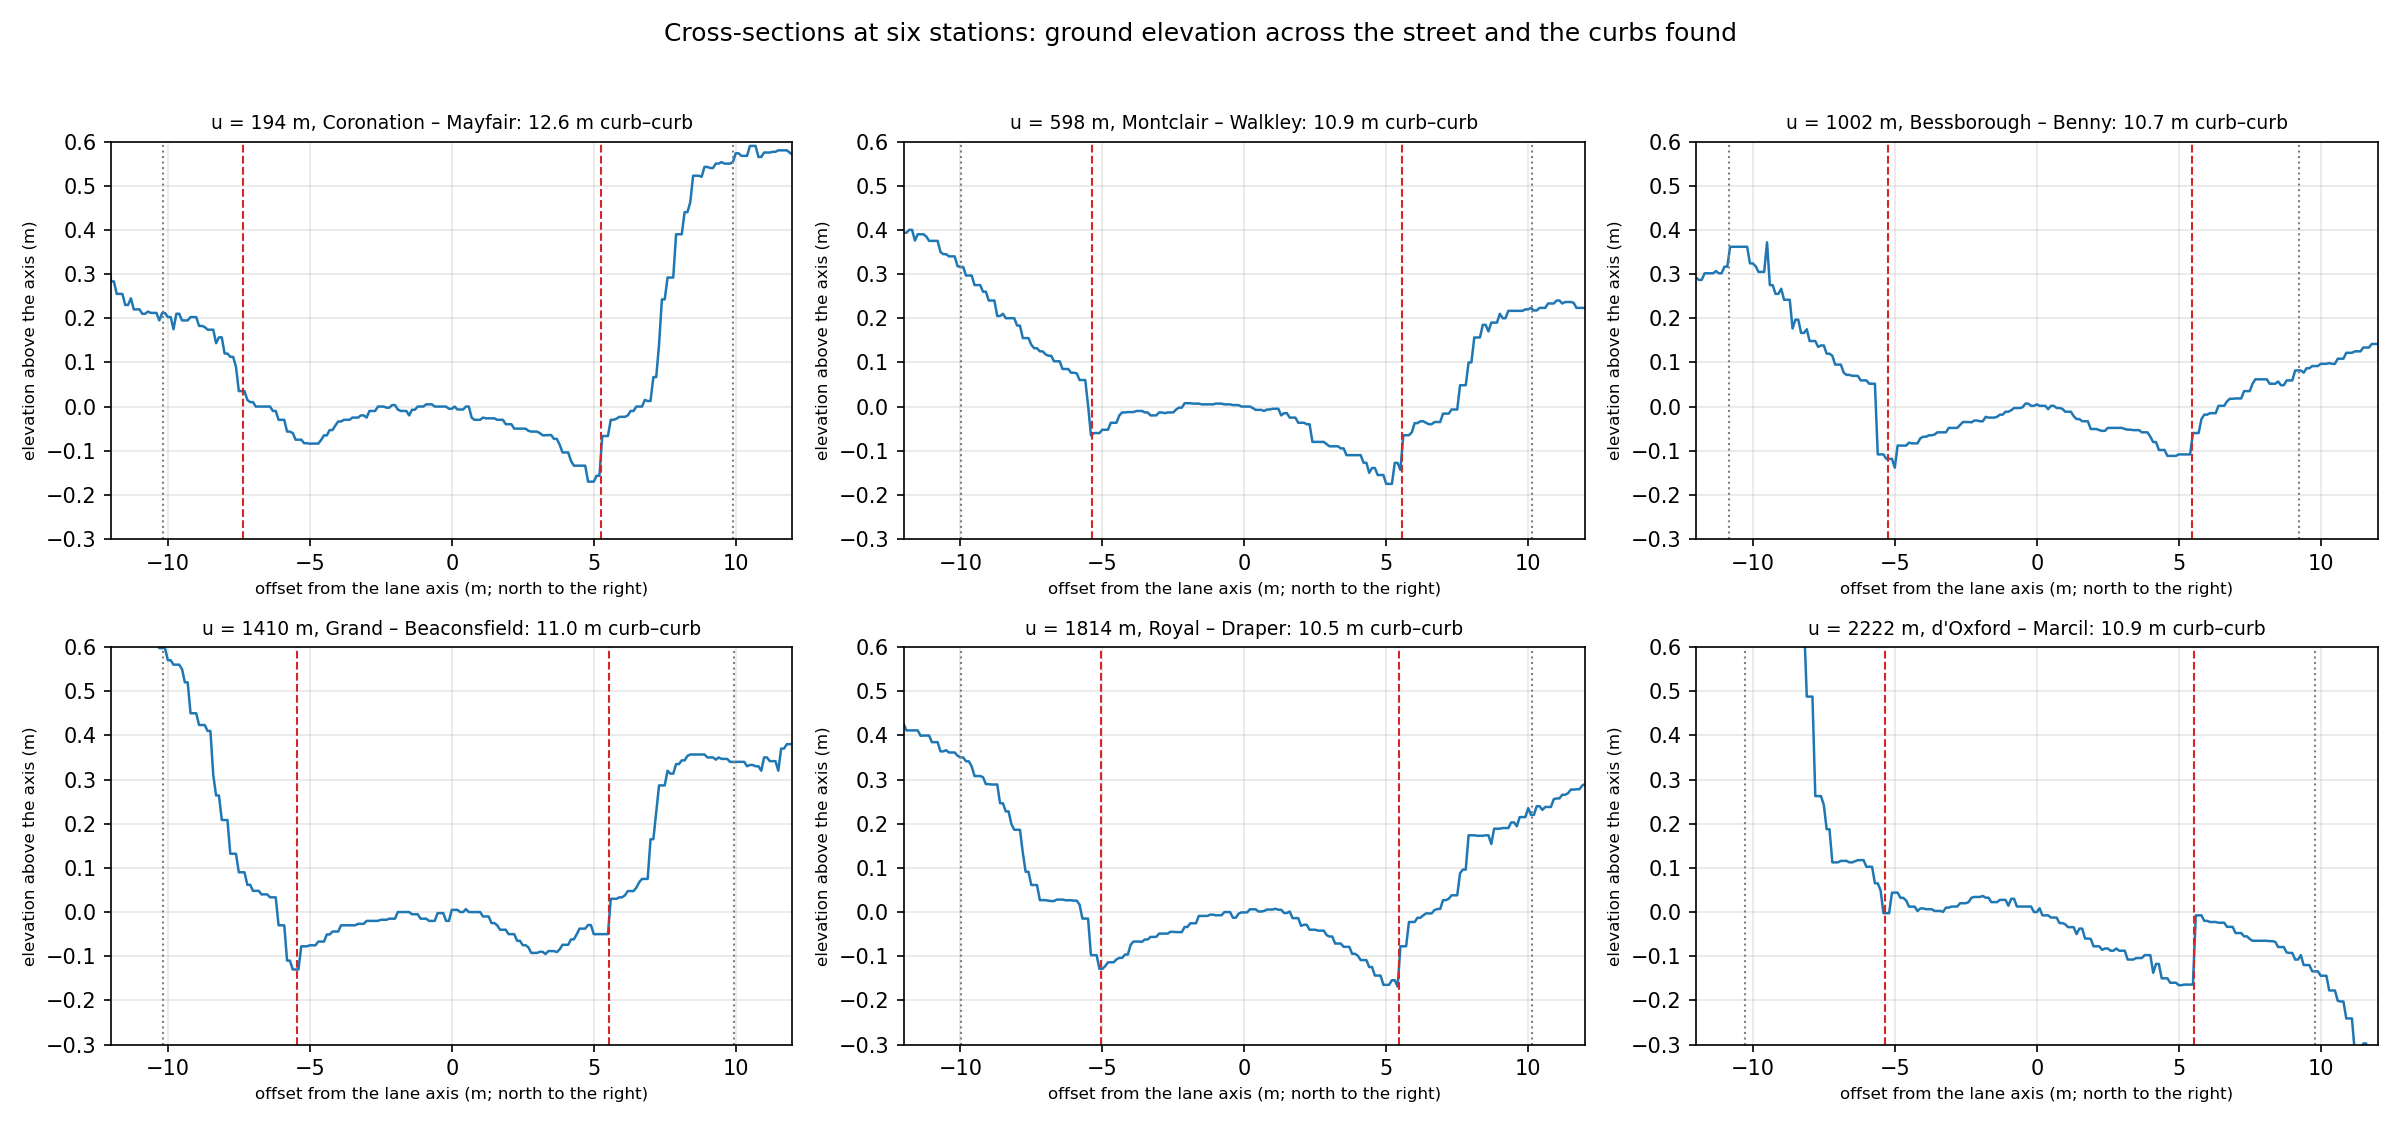
\includegraphics[width=\textwidth]{figures/street_width_sections_en.png}\end{frame}
\begin{frame}{Review: every curb detection on the LiDAR surface}\centering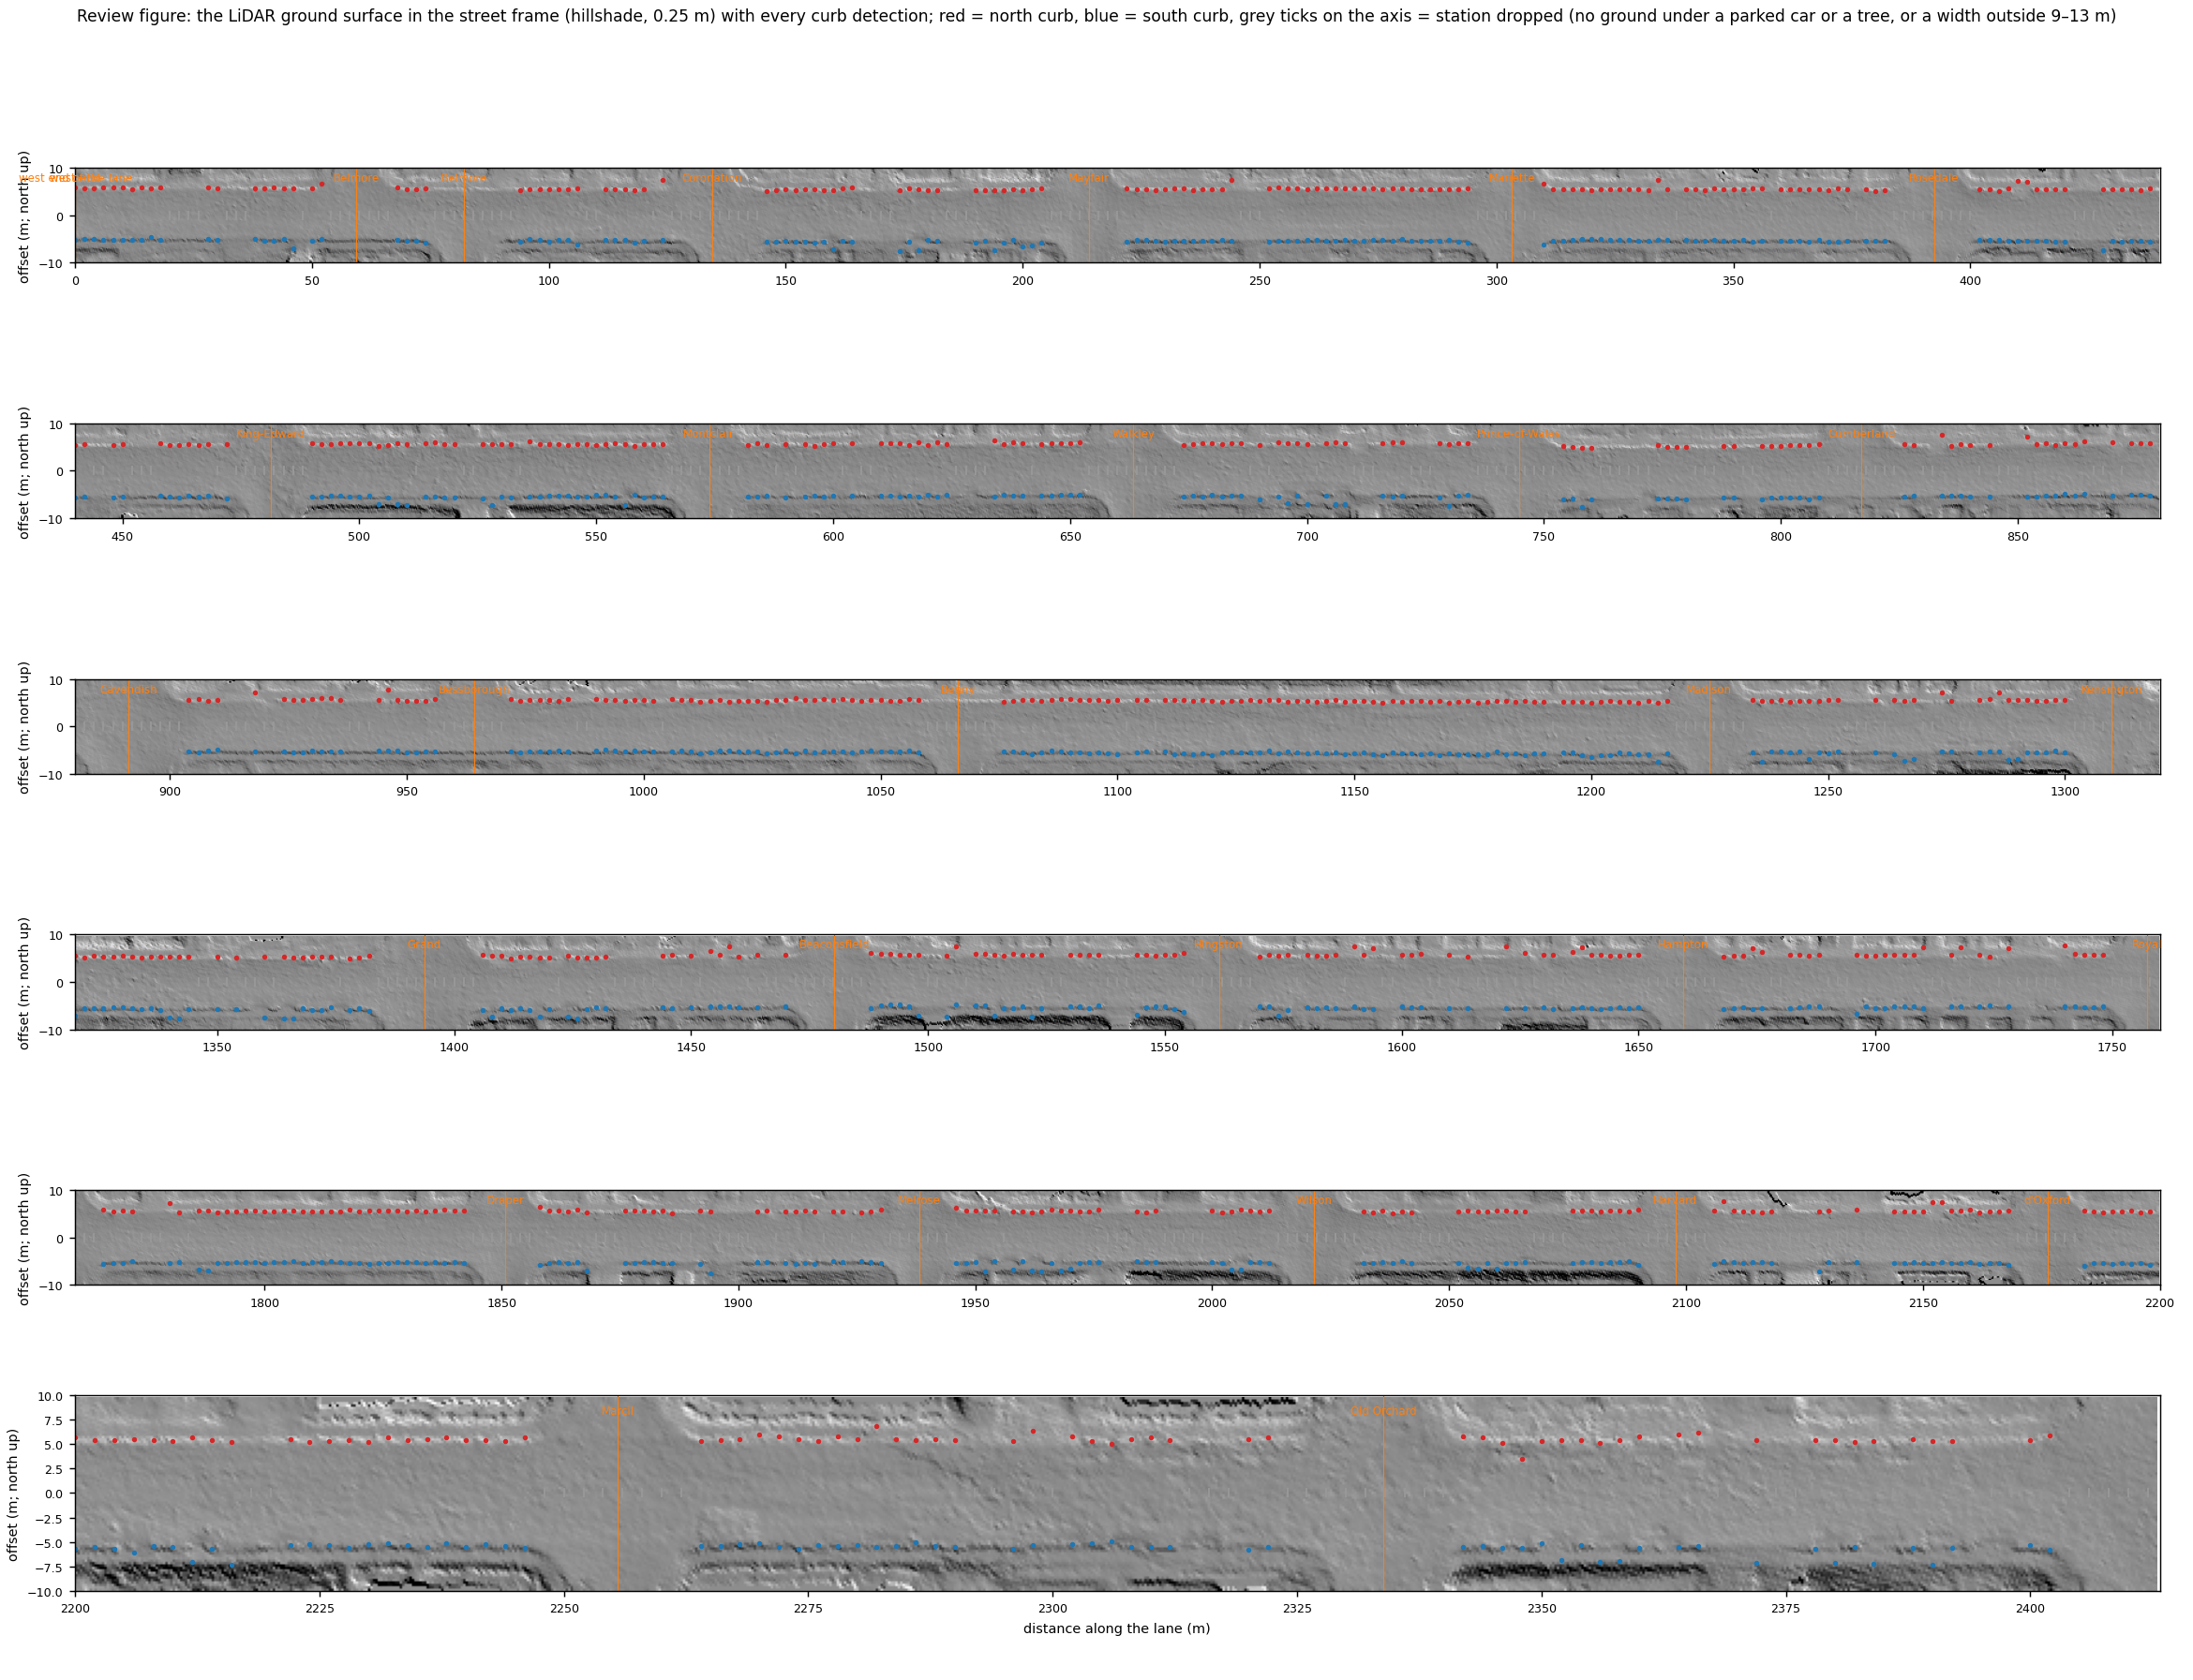
\includegraphics[height=0.86\textheight]{figures/street_width_overhead_en.png}\\{\tiny Hillshade of the ground surface in the street frame; red = north curb, blue = south curb; grey ticks on the axis = stations dropped (a parked car or a tree hid a curb, or the width fell outside 9--13 m).}\end{frame}
\begin{frame}{The west end, where the public street meets the Loyola campus}\centering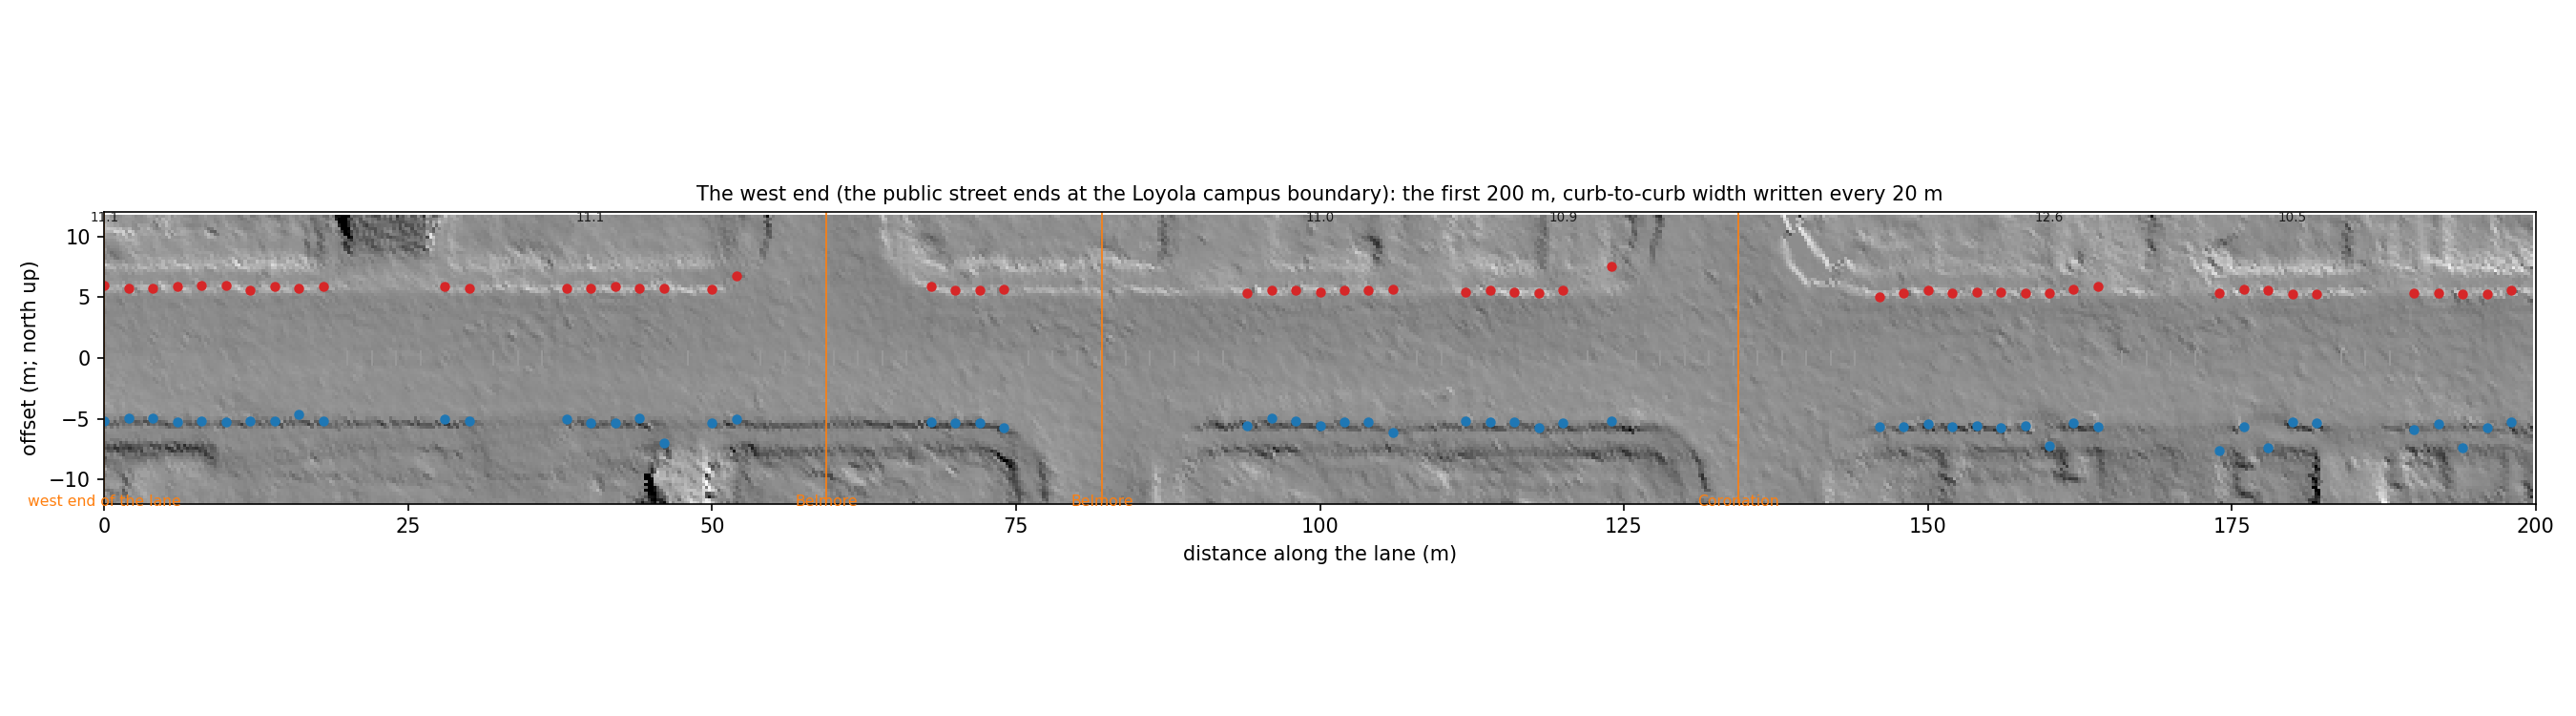
\includegraphics[width=\textwidth]{figures/street_width_west_end_en.png}\\{\small The last public block (west end to Belmore) reads 11.0 m curb to curb (19 of 30 stations), a 20.09 m right-of-way and 4.4--4.7 m sidewalk zones: the same section as the rest of the street. Beyond the lane\textquoteright{}s end the roadway is the campus\textquoteright{}s, not the City\textquoteright{}s (géobase). The 2015 surface and the pre-2024 imagery cannot measure the 2024 bike lanes themselves; a two-way block with no parking fits 11.0 m as, for example, 2.0 + 0.5 + 3.0 + 3.0 + 0.5 + 2.0 (arithmetic, not the plan).}\end{frame}
\begin{frame}{The figures}\begin{itemize}
\item Curb to curb: median \textbf{11.0 m} (p10 10.7, p90 12.4); block medians 10.8--11.35 m.
\item Right-of-way 20.09 m everywhere but the Belmore stub and three lots: the 66-foot standard.
\item Sidewalk zones, parcel line to curb: 4.4 m north, 4.73 m south.
\item EXP 2023 itself (p.~50): « une chaussée d\textquoteright{}environ 11 m et deux trottoirs d\textquoteright{}environ 1,8 m », 14.6 m in all: the LiDAR reconciles with the study\textquoteright{}s own measure.
\item Before 2024: two 3.3 m lanes and two 2.2 m parking bands = 11.0 m. Winter layout: 10.8 m of the 11.0 m.
\end{itemize}\end{frame}
\begin{frame}{What it means for the shared lane}\begin{itemize}
\item The 2023 drawing uses 10.8 of the 11.0 m: \textbf{about 0.2 m spare across the whole street}.
\item A shared lane wider than 3.5 m can only come from the parking bands (2.4 m), the buffer (0.5 m) or the contraflow lane (2.0 m).
\item With a cyclist 0.75 m wide at 0.5 m from the parked cars and the Code\textquoteright{}s 1 m clearance, 1.75 m of the shared lane is left for a car 1.8--2.0 m wide before mirrors (EXP Fig.~6-6; the owner\textquoteright{}s sketches). The width measured here does not change that arithmetic; it confirms the drawing\textquoteright{}s premise.
\item In winter, windrows push the parked cars toward the lane line: the measured 11.0 m is the summer maximum.
\end{itemize}\end{frame}
\begin{frame}{Caveats and where to find it}\begin{itemize}
\item One reading is good to about 0.2 m (0.25 m grid); use the block medians. Blocks with few kept stations carry more uncertainty.
\item 2015 surface, 2024 markings: the curbs have not moved; the markings are not in the LiDAR.
\item Every station, every block and the code: \url{https://openmobilitydata.github.io/Terrebonne-open-sources/2015-lidar-terrebonne-street-width/}
\end{itemize}\end{frame}
\end{document}
